\documentclass[12pt]{standalone}
\usepackage{tikz}
\usetikzlibrary{arrows.meta, positioning}

\begin{document}

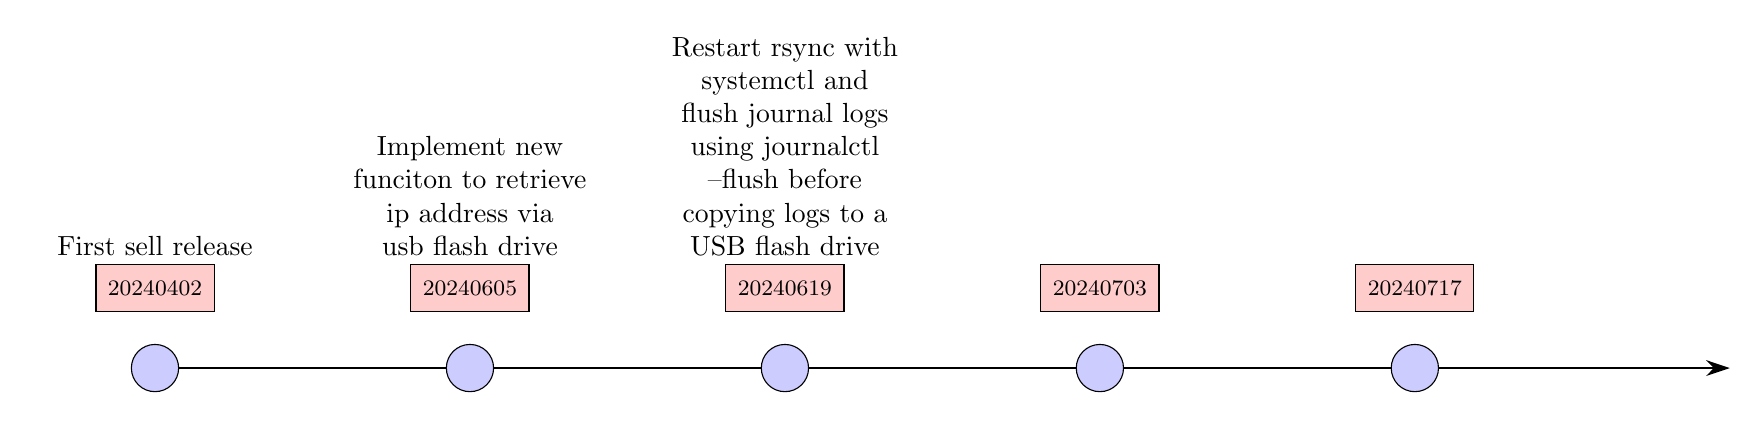
\begin{tikzpicture}[
    timeline/.style={
        thick,
        -{Stealth[length=3mm, width=2mm]}
    },
    milestone/.style={
        circle,
        draw=black,
        fill=blue!20,
        minimum size=6mm,
        inner sep=0pt
    },
    milestone label/.style={
        anchor=west,
        align=left,
        font=\footnotesize
    },
    version/.style={
        rectangle,
        draw=black,
        fill=red!20,
        minimum height=6mm,
        minimum width=15mm,
        inner sep=2pt,
        font=\footnotesize
    }
]

% Draw timeline
\draw[timeline] (0,0) -- (20,0);

% Add milestones and version labels
\foreach \x/\milestone/\version/\description in {
    00/{}/{20240402}/{First sell release},
    04/{}/{20240605}/{Implement new funciton to retrieve ip address via usb flash drive},
    08/{}/{20240619}/{Restart rsync with systemctl and flush journal logs using journalctl --flush before copying logs to a USB flash drive},
    12/{}/{20240703}/{},
    16/{}/{20240717}/{}
} {
    \node[milestone] (m\milestone) at (\x,0) {};
    \node[below=2mm of m\milestone, milestone label] {\milestone};
    \node[above=4mm of m\milestone, version] {\version};
    \node[above=10mm of m\milestone, align=center, text width=3cm] {\description};
}

\end{tikzpicture}

\end{document}


